\chapter{The HH$\rightarrow$4b analysis}

The search for the exact shape of the Higgs potential is an interesting endeavor as its not only  directly related to \ac{ewsb} but also could solve some fundamental questions about the nature of the universe as described in section \ref{sec:beyond_sm}. Since the Higgs interacts via Yukawa couplings from equation \ref{eq:yukawa_term} the coupling strengths for fermions are directly proportional to their mass and thus the Higgs couples most strongly to heavy particles. The main production modes at the \ac{lhc} are shown in figure \ref{fig:main_production_processes}. All couplings in the following are scaled with respect to their \ac{sm} values and are denoted with $\kappa_\mathrm{c} = c/c_\mathrm{sm}$ so that $\kappa_\mathrm{c}=1$ represents the \ac{sm} value of some coupling $c$.

The dominant Higgs pair production processes are shown in figure \ref{fig:main_production_processes}. The first two \ac{ggf} diagrams (a) and (b) have a cross-section of
$\sigma_\text{vbf HH}^\text{SM}=\qty[]{31.05}{fb}$ calculated at a center of mass energy of \qty[]{13}{TeV} at \ac{nnlo} \citep{Grazzini_2018} while the \ac{vbf} processes (c), (d) and (e) of figure \ref{fig:main_production_processes} have a production cross-section of
$\sigma_\text{vbf HH}^\text{SM}=\qty[]{1.73}{fb}$ at \ac{nnnlo} \citep{PhysRevD.98.114016}. A characteristic of the \ac{vbf} processes is that the Higgs pair products are accompanied by two additional quarks. The \ac{vbf} cross section is about \qty[]{3e4}{} times smaller than the production cross section for single Higgs $\sigma_\text{H}^\text{SM}=\qty[]{48.58}{pb}$ at the \ac{lhc} \citep{de2016arxiv} which already illustrates the challenge of discovering Higgs pairs in these final states.
\begin{figure}
    \centering
    \subfigure[]{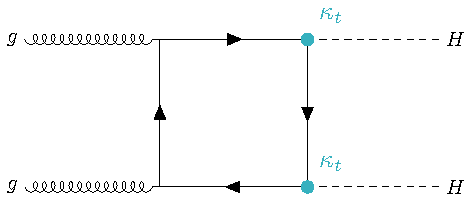
\includegraphics[width=.43\textwidth]{fig_01a}}\hspace{.06\textwidth}
    \subfigure[]{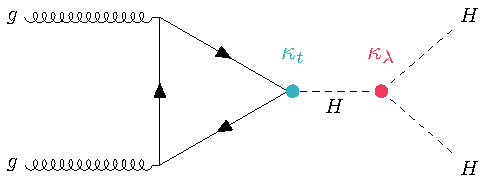
\includegraphics[width=.43\textwidth]{fig_01b}} \\
    \subfigure[]{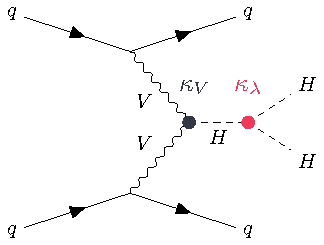
\includegraphics[width=.3\textwidth]{fig_02a}}\hspace{.01\textwidth}
    \subfigure[]{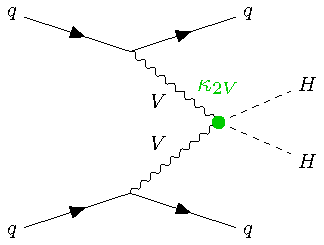
\includegraphics[width=.3\textwidth]{fig_02b}}\hspace{.01\textwidth}
    \subfigure[]{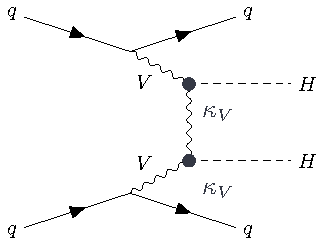
\includegraphics[width=.3\textwidth]{fig_02c}}
    \caption[]{Leading Higgs Pair production processes at the \ac{lhc}. (a), (b) shows \ac{ggf} and (c), (d), (e) \ac{vbf} processes. Adopted from \citep{aad2023search}.}
    \label{fig:main_production_processes}
\end{figure}
% higgs hat keine Ladung whatsoever cannot couple em or qcd 

\begin{figure}
    \centering
    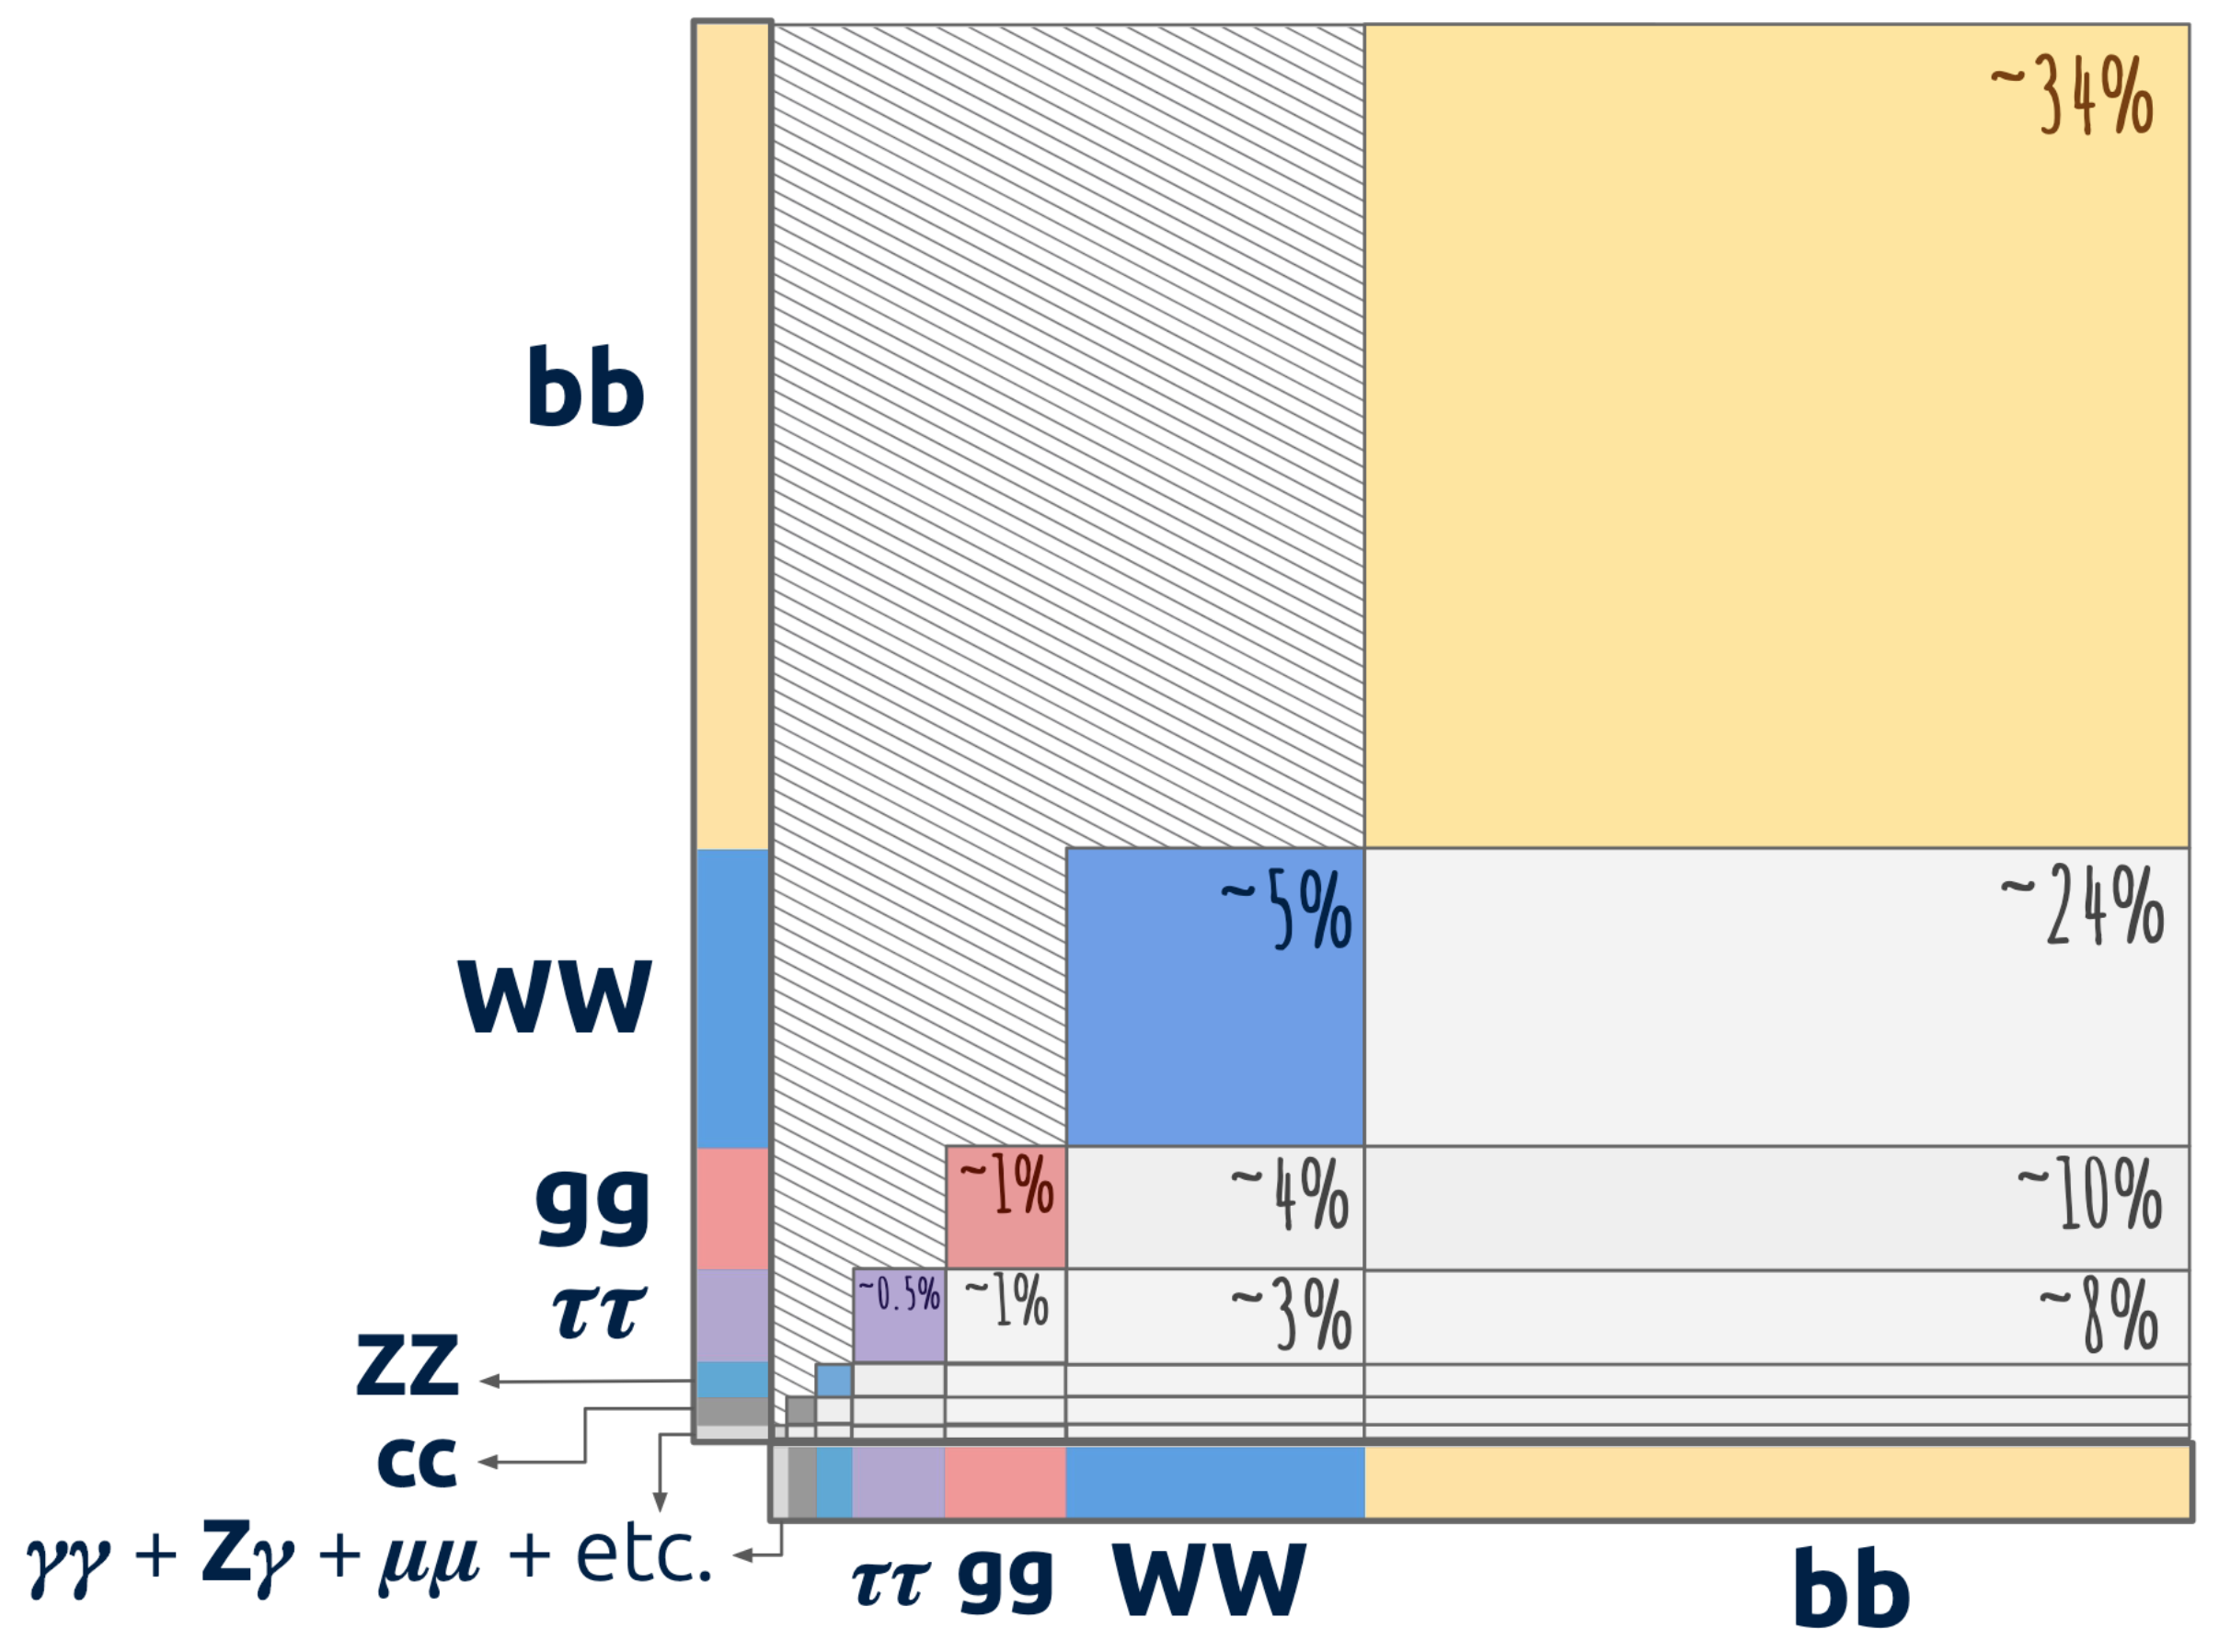
\includegraphics[width=0.7\textwidth]{branching_fraction_hh}
    \caption[]{Contributions of final states represented by area for a pair of Higgs. Adopted from \citep{ATL-COM-PHYS-2020-083}.}
    \label{fig:branching_fraction_hh}
\end{figure}
Figure \ref{fig:branching_fraction_hh} reveals that an interesting channel is the final state with the largest branching fraction of about \qty[]{34}{percent} consisting of four $b$-quarks. However as this a fully hadronic final state it comes with the challenge of large \ac{qcd} backgrounds.

This work focuses on the boosted topology of highly energetic jets which do not allow reconstruction of $b$-jets individually but rather of final states consisting of two collimated $b$-jets inside a larger jet. The advantage of this selection is that it reduces greatly the \ac{qcd} backgrounds since highly energetic jets aare more likely to come from heavy particles such as $b$ quarks. Furthermore it is easy to trigger on events containing jets with large \pt. Although they represent a comparatively clean signal such events are rare and therefore have limited statistical power. For this reason other search strategies are better suited for the discovery of the Higgs pair production process.

A reason for the low cross-section is that diagrams (d) and (e) of figure \ref{fig:main_production_processes} cancel each other destructively for \ac{sm} values. In turn if $\ktwov$ is moved to non-\ac{sm} values the production cross-section increases significantly $\sigma_{\ktwov=0}\approx 20\sigma_{\ktwov=1}$ \citep{bishara2017higgs} and the decay products have much larger transverse momentum as shown in figure \ref{fig:kappa_2v_variations_mhh}.
\begin{figure}
    \centering
    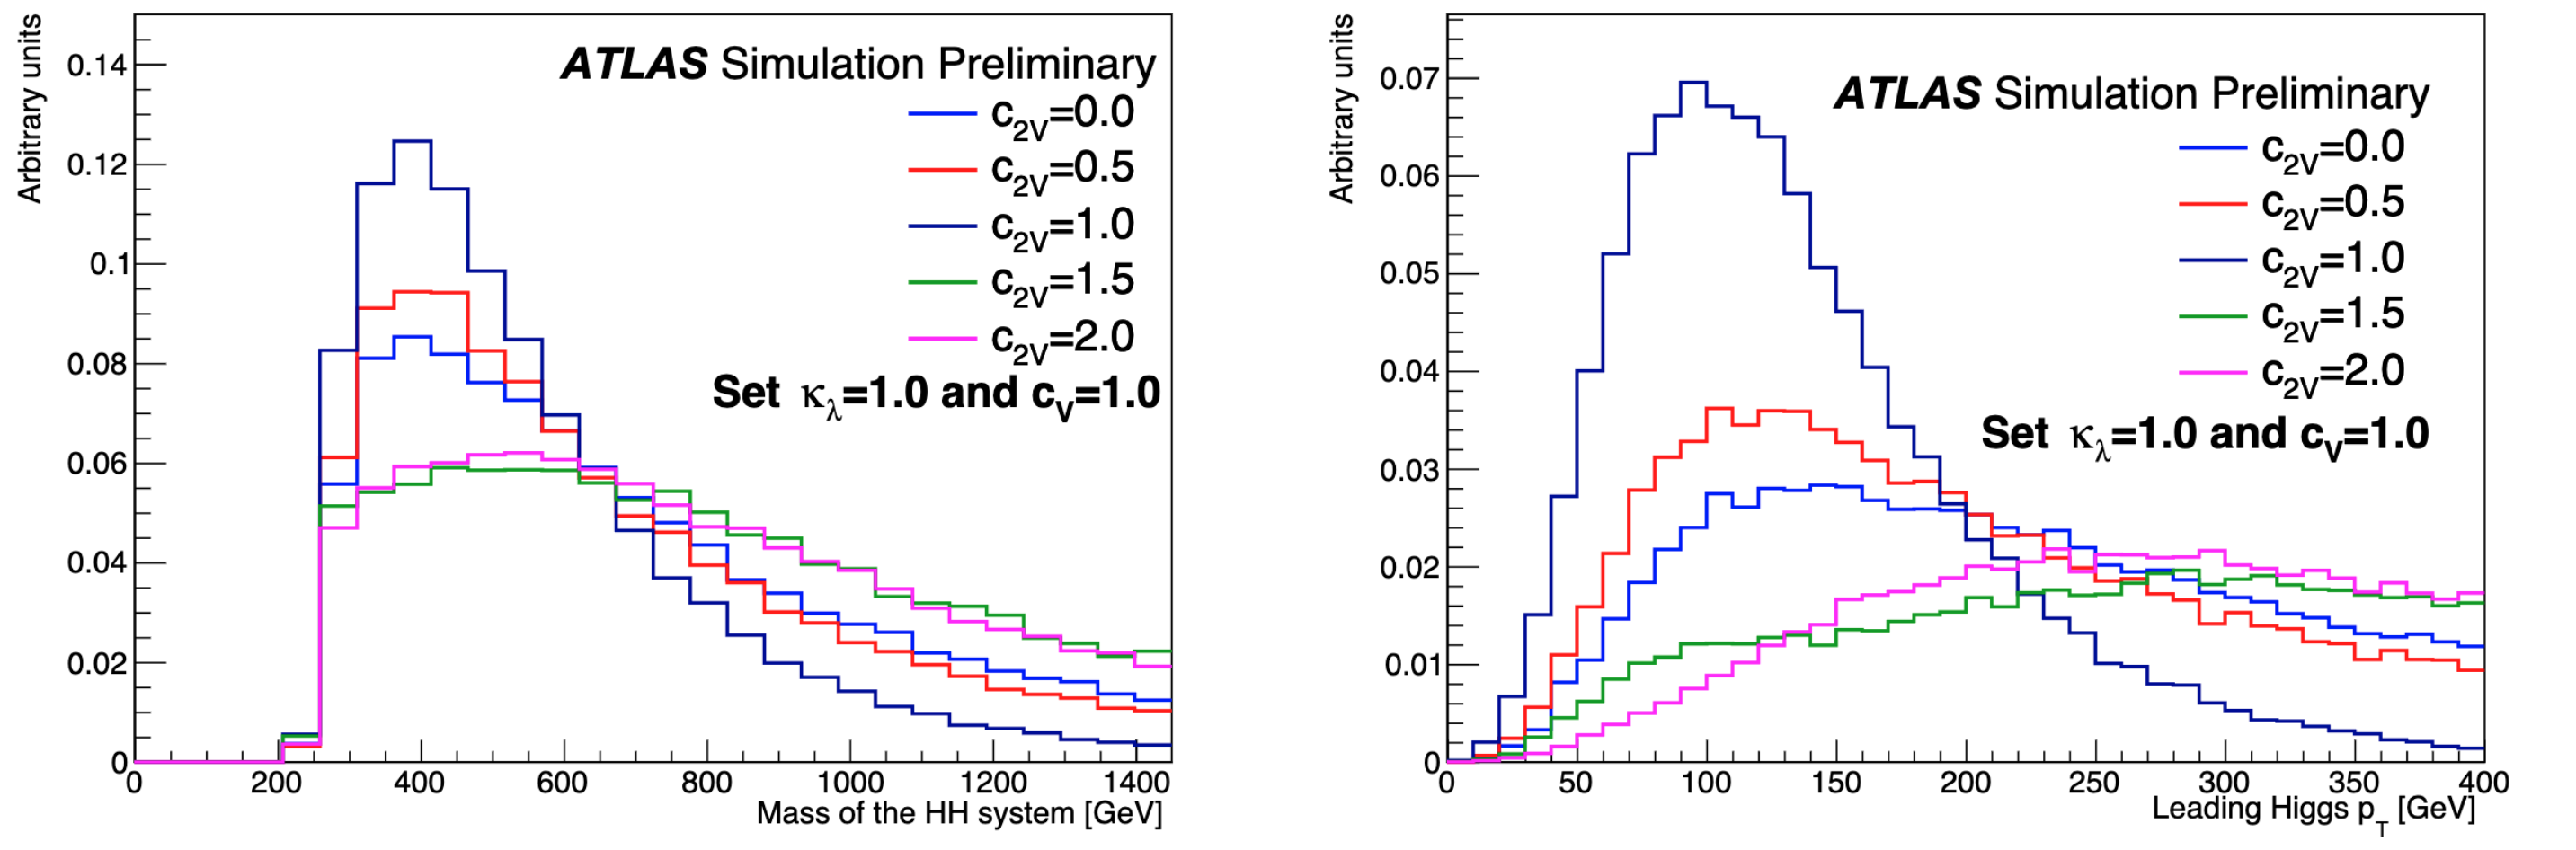
\includegraphics[width=1\textwidth]{kappa_2v_variations_mhh}
    \caption[]{Invariant mass of the Higgs pair system and the leading Higgs candidate jet \pt  reconstructed from simulation for different \ktwov. Adopted from \citep{ATL-PHYS-PUB-2019-007}.}
    \label{fig:kappa_2v_variations_mhh}
\end{figure}
Because of this behavior the power of this analysis lies in constraining and proving the existence of the \ktwov couplings within the \ac{sm} to which it is directly sensitive.

\section{Data and Monte Carlo Simulation}
This analysis uses the full run 2 data taken by \ac{atlas} between 2015 and 2018. The dataset contains \qty[]{140.1}{fb^{-1}} of data good for physics at a center of mass energy of \qty[]{13}{TeV} \citep{DAPR-2021-01}.

\ac{mc} generation in \ac{atlas} is done in three steps. At first at parton level events are generated with \textsc{MadGraph} (v.2.7.3p3.atlas6) \citep{alwall2014automated}. The output of this tool are stochastically sampled four vectors of the final states of the process of interest.

Afterwards the hadronization process is simulated with \textsc{Pythia8} \citep{Sjostrand:2014zea}.For this the \textsc{NNPDF3.0nlo} \ac{pdf} is used. The \ac{sm} \ac{vbf} cross-   section is rendered to the 4b branching ratio by multiplying it with $\mathcal{B}(4b)=0.3392$.


\red{add samples linear combination}
% https://www.overleaf.com/project/638e1930f926cd21d5264259
% linear combination
% Unfortunately, MC generation is computationally expensive and time-consuming. As such, only1443
% a handful of MC simulation samples for only a handful of coupling values are actually produced, and a1444
% sample combination technique is employed to model the signal hypothesis across the coupling parameter1445
% space
% https://trexfitter-docs.web.cern.ch/trexfitter-docs/model_building/expression/
% https://gitlab.cern.ch/hh4b/hh4b-boosted-vbf-limits/-/blob/main/create_workspaces/configs/k2V_parameterized_BDT_decorXbb.config?ref_type=heads#L285-331

\section{Analysis strategy}
This section describes the event selection and analysis strategy. A detailed description of reconstructed physical objects used is described in chapter \ref{ch:reco}.

\subsection{Trigger}
As outlined in section \ref{sec:tdaq} events need to be preselected/triggered. The \ac{hlt} applied in this analysis selects events with a large transverse energy $E_\text{T}$ large R jet. The definition slightly changed over the data taking years as can be seen in table \ref{tab:trigger}.
\begin{table}[htbp]
    \centering
    \caption{Trigger selections per data taking year and minimum requirements on transverse energy $E_\text{T}$ and mass $m$ on the large R jet. }
    \begin{tabular}{ccc}
        \hline
        Year & $E_\text{T}$ & $m$   \\ \hline
        2015 & $>360$       & 0     \\
        2016 & $>420$       & 0     \\
        2017 & $>420$       & $>35$ \\
        2018 & $>420$       & $>40$ \\ \hline
    \end{tabular}
    \label{tab:trigger}
\end{table}
Previous studies have shown that they become fully efficient at about $\pt>\qty[]{420}{GeV}$ \citep{ATL-COM-PHYS-2020-083,ATL-COM-PHYS-2023-033}.
% \red{Figure \ref{fig:trigger_eff} depicts the efficiencies for the different triggers that become fully efficient at about $\pt>\qty[]{420}{GeV}$}.
% \begin{figure}
%     \centering
%     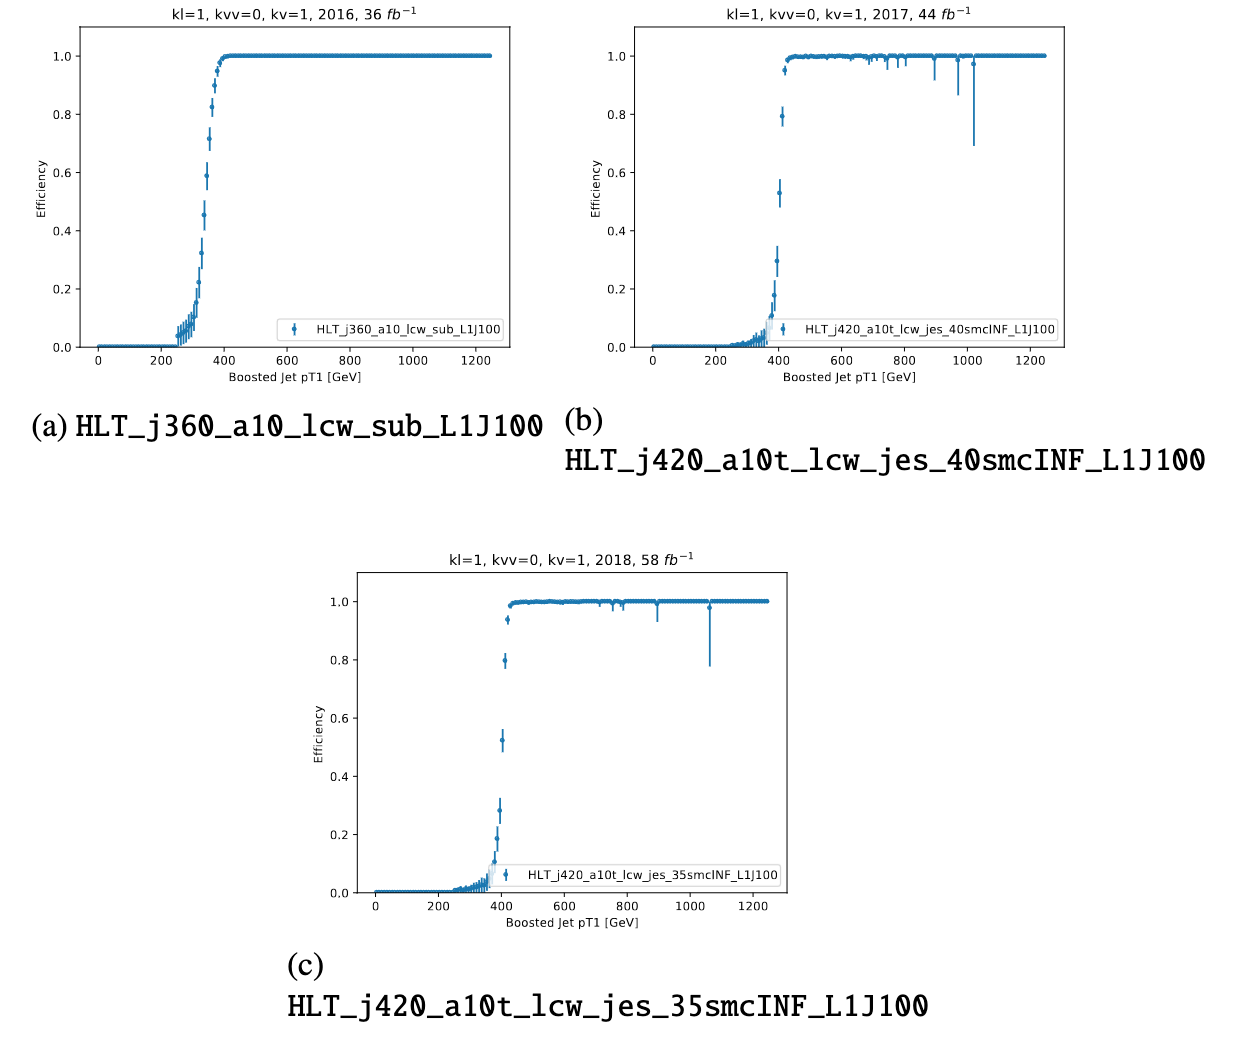
\includegraphics[width=1\textwidth]{trigger_eff}
%     \caption[]{\red{TODO MYSELF}}
%     \label{fig:trigger_eff}
% \end{figure}

\subsection{Large Radius Jets}
To fully capture the boosted Higgs pair topology two large $R=1.0$ jets clustered with the Anti-$k_t$ algorithm from \acp{tcc} are used as described in section \ref{sec:jets}. These enclose the two boosted collimated $b$-jets in each of them to form the Higgs candidates. If there are several large-$R$ jets the two with the highest \pt are chosen. To be fully efficient on the trigger the leading large-$R$ jet is required to have $\pt>\qty[]{450}{GeV}$. In general for decay products to be inside a jet approximately holds $R\approx 2m/\pt$ with the mass $m$ and tranverse momentum of the parent particle \citep{ATL-COM-PHYS-2020-083}. For a Higgs mass of \qty[]{125}{GeV} to be contained inside a large-$R$ jet the Higgs candidate therefore must have $\pt\gtrsim \qty[]{250}{GeV}$ and is thus chosen as the \pt requirement on the sub-leading Higgs candidate. Additionally both Higgs candidates have a mass requirement $m>\qty[]{50}{GeV}$ to reduce \ac{qcd} background.

% As a minimum quality criterion large R jets are then required to have $200<p_{\text{T}}<3000$ GeV, $50<m<600$ GeV and $|\eta|<2$.

The identification of $b$-jets inside the selected large-$R$ jets is done with the $X\rightarrow bb$ tagger explained in section \ref{sec:xbb}. The top fraction $f_\text{top}$ is set to 0.25 and the \qty[]{60}{\percent} Higgs efficiency \ac{wp} is required. Studies with the more inclusive \qty[]{60}{\percent} \ac{wp} displayed slightly worse limit results \citep{ATL-COM-PHYS-2023-033}.

\subsection{Small Radius Jets}
Two small radius $R=0.4$ jets are required for the \ac{vbf} signature and are referred to as \ac{vbf} jets in the following. They are also reconstructed with the anti-$k_t$ algorithm and as \acp{pfo} as described in \ref{sec:jets}. The tight \ac{wp} for the \ac{jvt} ad the LooseBad \ac{wp}for the event cleaning are applied both described in \ref{sec:calibration}. Small-$R$ jets $j$ are selected for $\pt>\qty[]{20}{GeV}$ and $|\eta|<4.5$ and are required to be outside of the Higgs candidate large-$R$ jets $J$ by imposing $\Delta R(J,j) > 1.4$. \red{Further cuts applied on the jet system optimized on significance are $|\Delta\eta(j,j)| > 3$ and $m_{jj} > \qty{1}{TeV}$.}

\subsection{Kinematic Regions}\label{sec:kinematic_regions}
\ac{sr},\ac{vr} and \ac{cr} are explored and optimized in previous analyses \citep{aad2023search,ATL-COM-PHYS-2023-033} in the $m_{H1},m_{H2}$ plane and are defined as
\begin{equation}
    SR=X_{hh} =  \sqrt{\left(\frac{m_{H1} - \SI{124}{\GeV}}{1500 / m_{H1}}\right)^{2} + \left(\frac{m_{H2} - \SI{117}{\GeV}}{1900 / m_{H2}}\right)^{2}} < 1.6,
\end{equation}
\begin{equation}
    \label{VR_Xhh}
    VR =  \sqrt{\left(\frac{m_{H1} - \SI{124}{\GeV}}{0.1 \ln(m_{H1})}\right)^{2} + \left(\frac{m_{H2} - \SI{117}{\GeV}}{0.1 \ln(m_{H2})}\right)^{2}} < 100,
\end{equation}
and
\begin{equation}
    \label{CR_Xhh}
    CR = \sqrt{\left(\frac{m_{H1} - \SI{124}{\GeV}}{0.1 \ln(m_{H1})}\right)^{2} + \left(\frac{m_{H2} - \SI{117}{\GeV}}{0.1 \ln(m_{H2})}\right)^{2}} > 100  \ \& \ < 170.
\end{equation}
Figure depicts the regions in the $m_{H1},m_{H2}$ plane on the \ac{sm} signal sample

\begin{figure}
    \centering
    \subfigure[]{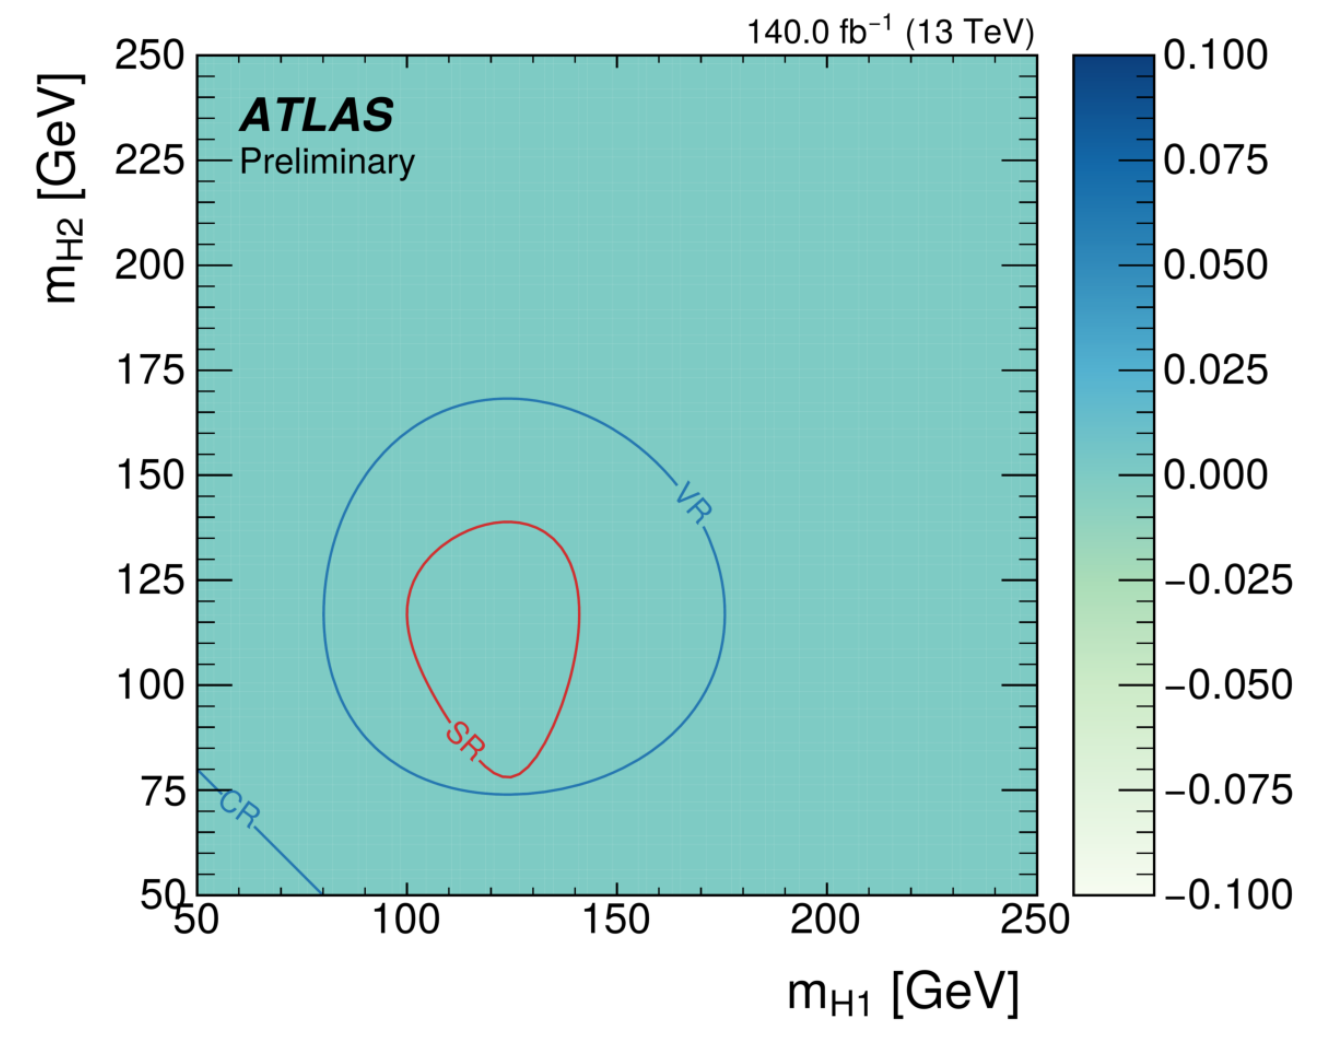
\includegraphics[width=.49\textwidth]{m_hh_plane}}
    \subfigure[]{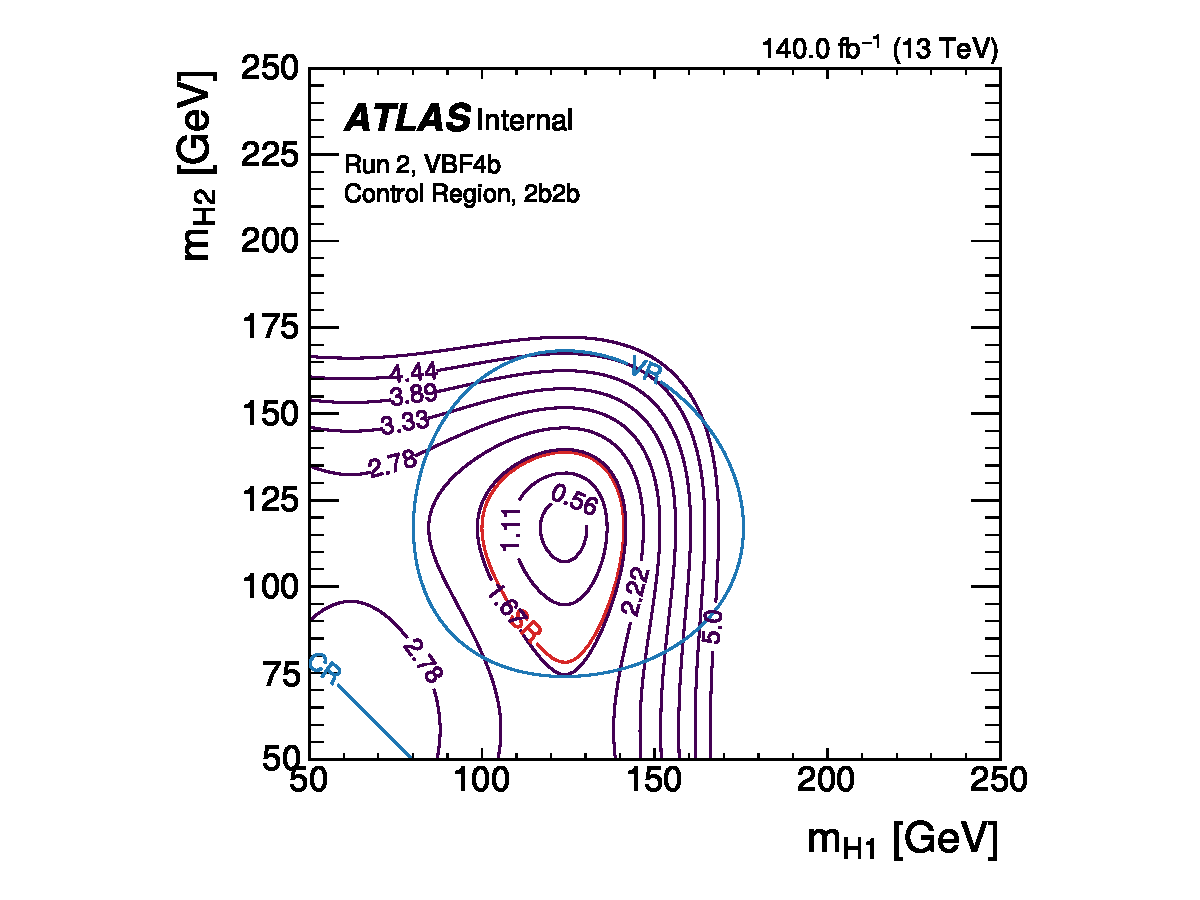
\includegraphics[width=.49\textwidth]{massplane_SR_opening}}
    \caption[]{\red{REDO}}
    \label{fig:m_hh_plane}
\end{figure}
\subsection{Cutflow}
\red{TODO, also fine like that?}
\red{
    \begin{table}[ht]
        \centering
        \begin{tabular}{lccc}
            \hline  \hline
            Selection                          & Event           & Fraction [\%] & Total Fraction [\%] \\
            \hline  \hline
            Initial                            & 16854036422.000 &               &                     \\
            Preselections (MNT + Jet Cleaning) & 670573995.000   & 100.000       & 100.000             \\
            PassTrigBoosted                    & 63944638.000    & 9.536         & 9.536               \\
            PassTwoFatJets                     & 57510800.000    & 89.938        & 8.576               \\
            PassTwoHbbJets                     & 12875.000       & 0.0223        & <0.001              \\
            PassVBFJets                        & 5762.000        & 44.753        & <0.001              \\
            PassFatJetPt                       & 3902.000        & 67.720        & <0.001              \\
            PassVBFCut                         & 314.000         & 8.047         & <0.001              \\
            \hline  \hline
        \end{tabular}
        \caption{Cut-flow table for data before signal region cut}
        \label{cutflow_dsid502970}
    \end{table}
}


\begin{table}[ht]
    \centering
    \begin{tabular}{lccc}
        \hline  \hline
        Selection                          & Event    & Fraction [\%] & Total Fraction [\%] \\
        \hline  \hline
        Initial                            & 1475.226 &               &                     \\
        Preselections (MNT + Jet Cleaning) & 547.960  & 100.000       & 100.000             \\
        PassTrigBoosted                    & 20.926   & 3.819         & 3.819               \\
        PassTwoFatJets                     & 14.141   & 67.576        & 2.581               \\
        PassTwoHbbJets                     & 5.353    & 37.852        & 0.977               \\
        PassVBFJets                        & 2.243    & 41.903        & 0.409               \\
        PassFatJetPt                       & 1.408    & 62.793        & 0.257               \\
        PassVBFCut                         & 0.148    & 10.539        & 0.027               \\
        PassSR                             & 0.097    & 65.484        & 0.018               \\
        OverlapRemoval                     & 0.059    & 61.200        & 0.011               \\
        \hline  \hline
    \end{tabular}
    \caption{Cut-flow table for DSID = 600463}
    \label{cutflow_dsid600463}
\end{table}

\red{\subsection{Analysis Optimization}
present here the used NN, retrieved from neos from chapter blah 
}
\subsection{Background Estimation}
Since the final state of this analysis is hadronic it remains an infeasible task to estimate the contributions from the plethora of \ac{qcd} processes that contribute to the background. Therefore the well established ABCD method is employed to derive a data-driven background estimate \citep{buttinger2018background,PhysRevD.103.035021}. Its is based on the idea to use two independent variables e.g. $f$ and $g$ to define four orthogonal regions A,B,C and D as illustrated in figure \ref{fig:abcd} so that for some combination of the ratio of the event yields in the regions hold
\begin{equation}
    \frac{N_A}{N_B}=\frac{N_C}{N_D}.
\end{equation}
\begin{figure}
    \centering
    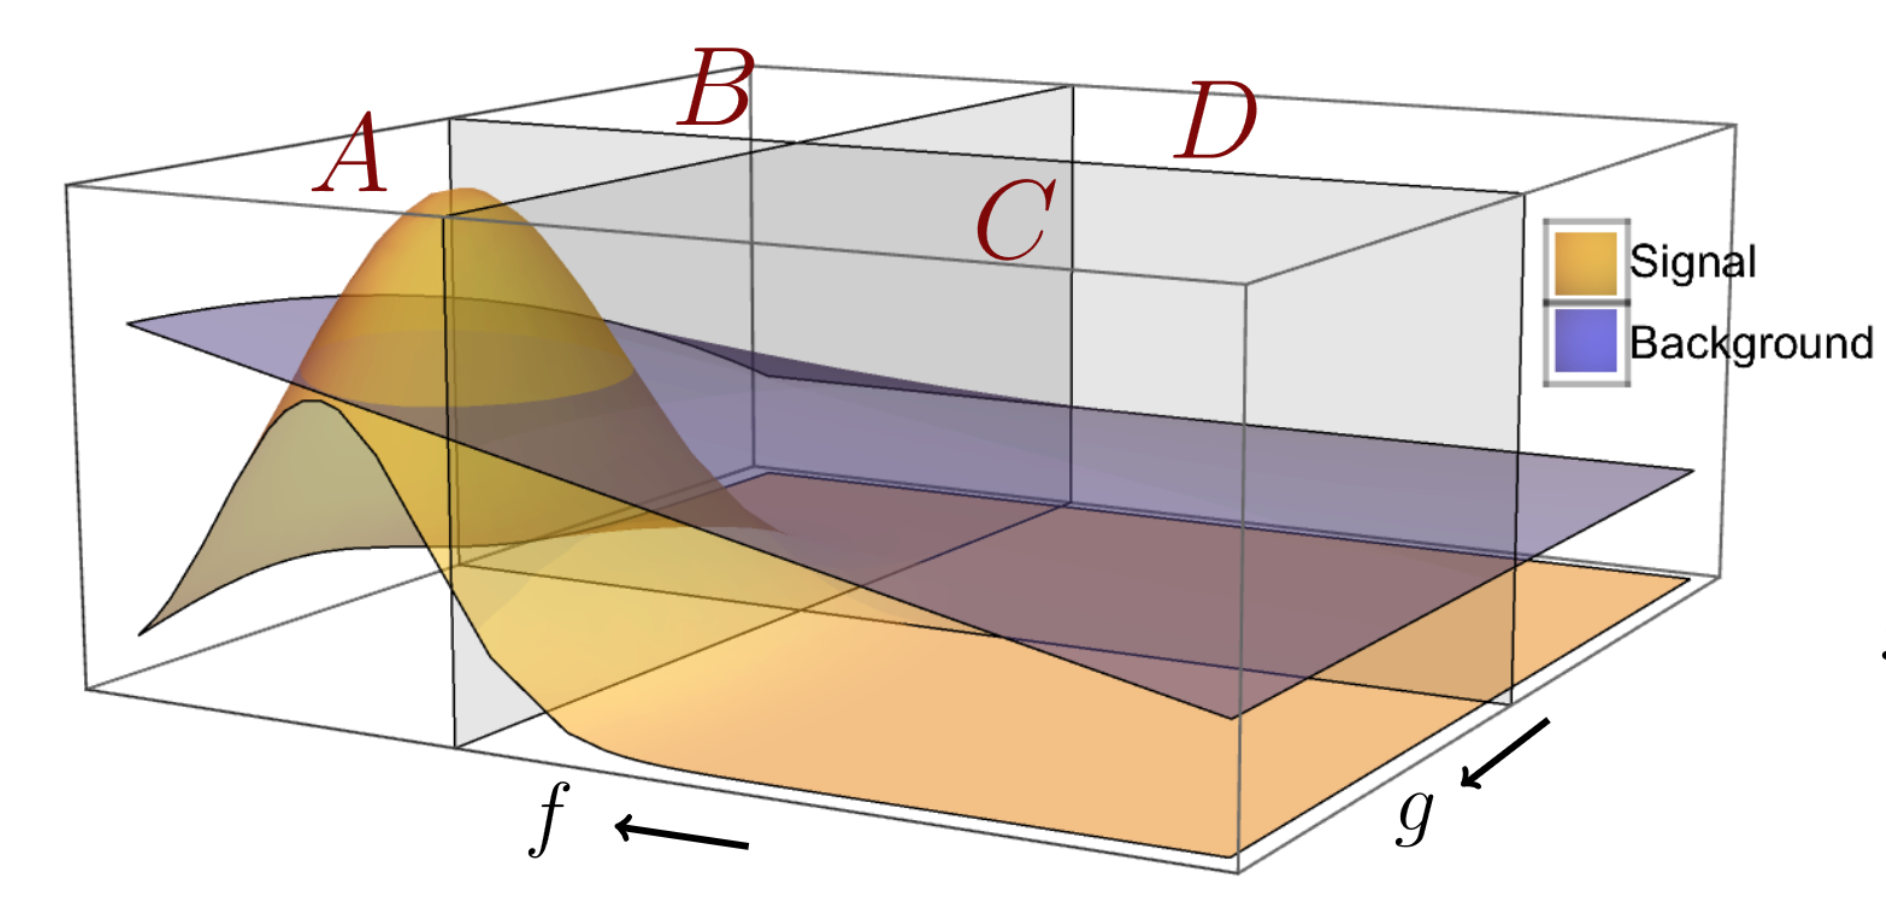
\includegraphics[width=.7\textwidth]{abcd}
    \caption[]{Illustration of four orthogonal regions A,B,C and D defined by two variables $f$ and $g$ in the horizontal and signal and background yields in the vertical dimension. Adopted from \citep{PhysRevD.103.035021}.}
    \label{fig:abcd}
\end{figure}
By rearranging the equation for the unknown $N_A$ an estimate for the background of the signal region can be derived from the other known quantities that lie in the regions dominated by the background. This approach only works well if the change in shape of the background in Figure \ref{fig:abcd} does not vary greatly between C to D and A to B. Therefore the method should always be tested in another region to proof its validity.

In this analysis the two orthogonal variables are defined via the amount of $X\rightarrow bb$ Higgs tagged large-$R$ jets denoted as Xbb and the kinematic regions of the \ac{sr} and \ac{cr} defined in \ref{sec:kinematic_regions}.
\begin{table}[htbp]
    \centering
    \caption{Four orthogonal region definitions for the ABCD method}
    \begin{tabular}{|c|c|}
        \hline
        2 Xbb in CR & 2 Xbb in SR \\ \hline
        1 Xbb in CR & 1 Xbb in SR \\ \hline
    \end{tabular}
    \label{tab:abcd}
\end{table}
This gives the four orthogonal regions shown in table \ref{tab:abcd} so that the background in the \ac{sr} is estimated with a weight extracted from the \ac{cr}
\begin{equation}
    N_\text{SR}^\text{2Higgs}=\frac{N_\text{CR}^\text{2Higgs}}{N_\text{CR}^\text{1Higgs}} N_\text{SR}^\text{1Higgs} = w_\text{CR} N_\text{SR}^\text{1Higgs}.
\end{equation}

\red{question is if we put the validation already here, conflict with neos description, beacuse would need to explain the nn used before to understand validation}

\red{studies with a bin-wise trained \ac{nn} didnt gain anything (like in the resolved analysis), but lets put this as well in the results part}